\documentclass[12pt,letterpaper]{article}
\usepackage[latin1]{inputenc}
\usepackage{amsmath}
\usepackage{amsfonts}
\usepackage{amssymb}
\usepackage{graphicx}
\usepackage{caption}

\graphicspath{{./plots/}}
\begin{document}
{\centering
\title{Growing Degree Day Project \\ \vspace{.5 cm} {\Large Computer Based and Application Tools Course Project} }
\maketitle
%\author{Ozair Shafiq ~ Farhad M. Kazemi ~ Yeni Liang ~ Minhaj Shunjaruff \\ Zahed khatooni ~  Silvana Pereira ~  Ibrahim Alonge}

{\itshape Memorial University of Newfoundland \\ St. John's, Canada.\par}
}
\begin{abstract}
The aim of this research is to find the...

The results showed that...
\end{abstract}

\section{Introduction}

In this report, we would like to...
\\
\begin{equation}
\textrm{GDD} = \left(\frac{T_{max} + T_{min}}{2}\right) - T_{base}
\label{eqn:gdd}
\end{equation}
\\
On the rest of this report, firstly we will describe our dataset properties and what we have done to clean this data and to overcome data heterogeneity and missing values. In the second section, we briefly described ....
Finally, we have a conclusion and what could be done in the future works.
\section{Question 1:Dealing With Dataset}
Prerequisite of this script is a text file that will contain two strings separated by a comma on each line. The left string specifies the station name or its sub-name, the right string specifies the province that this station may belong to. The script takes the left string and searches it in Station Inventory EN file at Historical Climate data service provided by the government of Canada. It will fetch daily temperatures for stations that either match completely with the left string or sub-matches with the left string. For example, if the left string is 'toronto', all stations names in Station Inventory EN that contain the string 'toronto' will be matched by the script  and if the data is available for the specific years asked by the user, then its daily data for each of those years will be downloaded. The script will then combine all this data, sort the data date-wise and write this to a '/data' folder for convenience, for each line in the text file.\\
The program will also generate another text file that will contain the latitudes and longitudes for each location specified in the input text as the coordinates of that station that occupies the most years in the requested time-line.\\
Hence, the program requires two command line arguments, a text file containing station name, province pair in each line and Year specified as 'yyyy' that specifies the time-line as 2016-Year. For example, if 2012 is provided as the year, the program will fetch data for 2012 till 2016 time-line.

\section{Question 2}
\section{Question 3}
Write a command line program that takes arguments.\\
\section{Question 4}
\section{Question 5}
\section{Question 6}
\section{Question 7}
\section{Question 8}
\section{Question 9}
\section{Question 10}
\section{Question 1 optional}
\section{Question 2 optional}
\section{Question 3 optional}
=======
\section{Question 3}
Write a command line program that takes arguments\\
In the GDD calculation part, we have used the package argparse to handle the command line arguments. First, we set the csv argument which completes file path of cities file. Second, we set the tbase argument (default = 10) and tupper argument(default = 30) to apply in the GDD calculation.\\
The data needed for GDD calculation are already downloaded and stored in the data folder with their filenames specified in citiex.txt file. In this program, it read these data directly from data folder, do calculation on each file, and store them separately. For the missing information in csv file, we will set the GDD to 0. The GDD calculation equation is below:

In our program, we set the $ T_max$ value to the minimum between tupper and the maximum daily temperature and $ T_base$ to the 10. For example, on 15th, August, 2010 in Vancouver, the maximum temperature is 31.2 Celsius degrees which is more than 30 Celsius degrees, and the minimum temperature is 16.1 Celsius degrees. Hence the GDD equation to $(\frac{30+16.1}{2})-10$  
and the GDD result is $13.05$ .
Finally, we add the new GDD column to the existing data files, which is supposed to prevent creating more files in the project.
In the next part, we are supposed to use the GDD calculation to create plots showing accumulated GDD vs time for selected cities.

\begin{figure}
\centering
\includegraphics[scale=0.6]{{"st. john's,newfoundland_MinMax"}.png}
\caption{D}
\end{figure}

\begin{figure}
\centering
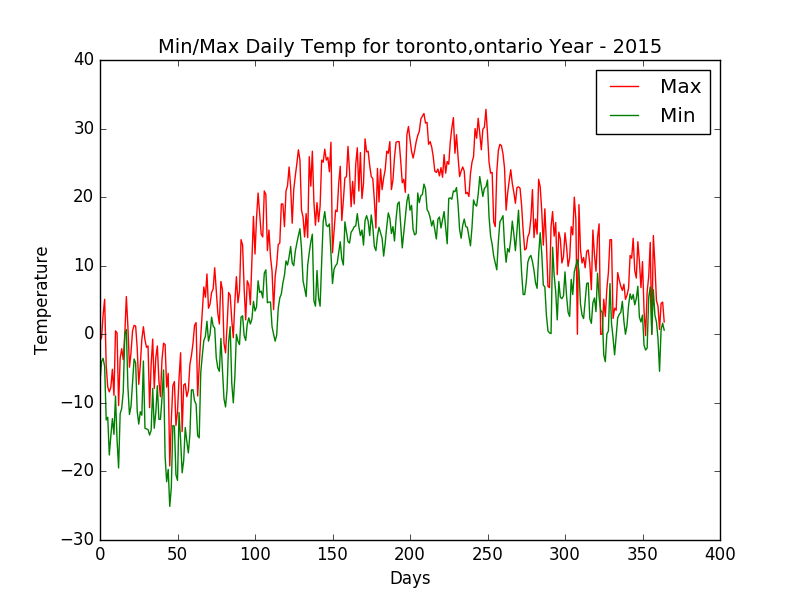
\includegraphics[scale=0.6]{toronto,ontario_MinMax.png}
\caption{E}
\end{figure}

\begin{figure}
\centering
\includegraphics[scale=0.6]{{"vancouver,british columbia_MinMax"}.png}
\caption{F}
\end{figure}

\begin{figure}
\centering
\includegraphics[scale=0.6]{{"st. john's,newfoundland_GddPlot"}.png}
\caption{A}
\label{fig:gbm}
\end{figure}

\begin{figure}
\centering
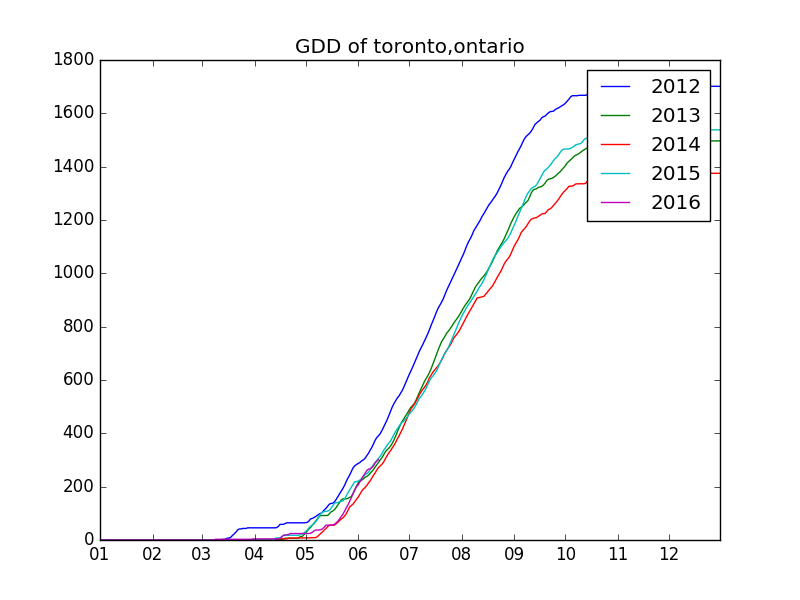
\includegraphics[scale=0.6]{toronto,ontario_GddPlot.png}
\caption{B}
\label{fig:gbm}
\end{figure}

\begin{figure}
\centering
\includegraphics[scale=0.6]{{"vancouver,british columbia_GddPlot"}.png}
\caption{C}
\end{figure}

\begin{figure}
\centering
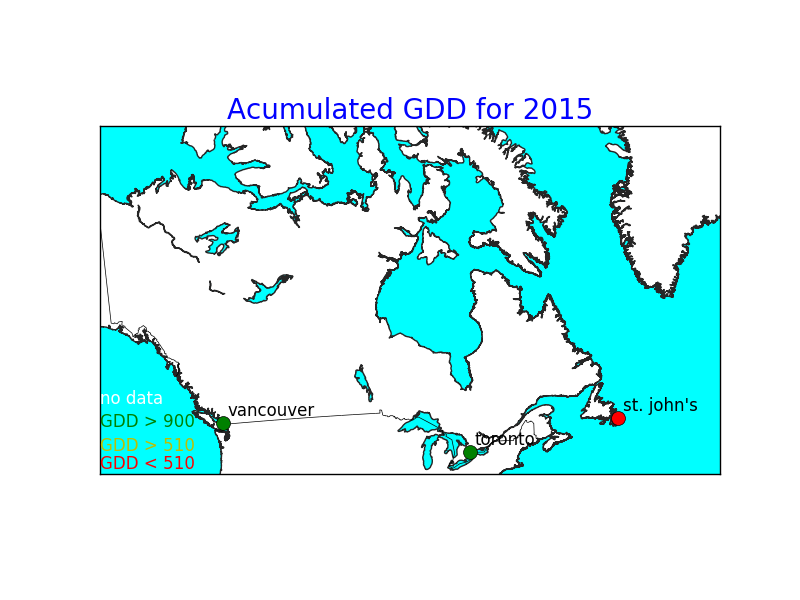
\includegraphics[scale=0.6]{GDDMap_2015.png}
\caption{F}
\end{figure}

\begin{figure}
\centering
\includegraphics[scale=0.6]{{"st. john's,newfoundland_Tbase_GddPlot"}.png}
\caption{C}
\end{figure}

\begin{figure}
\centering
\includegraphics[scale=0.6]{{"toronto,ontario_Tbase_GddPlot"}.png}
\caption{C}
\end{figure}

\begin{figure}
\centering
\includegraphics[scale=0.6]{{"vancouver,british columbia_Tbase_GddPlot"}.png}
\caption{C}
\end{figure}


%\includegraphics{plot00.png}
%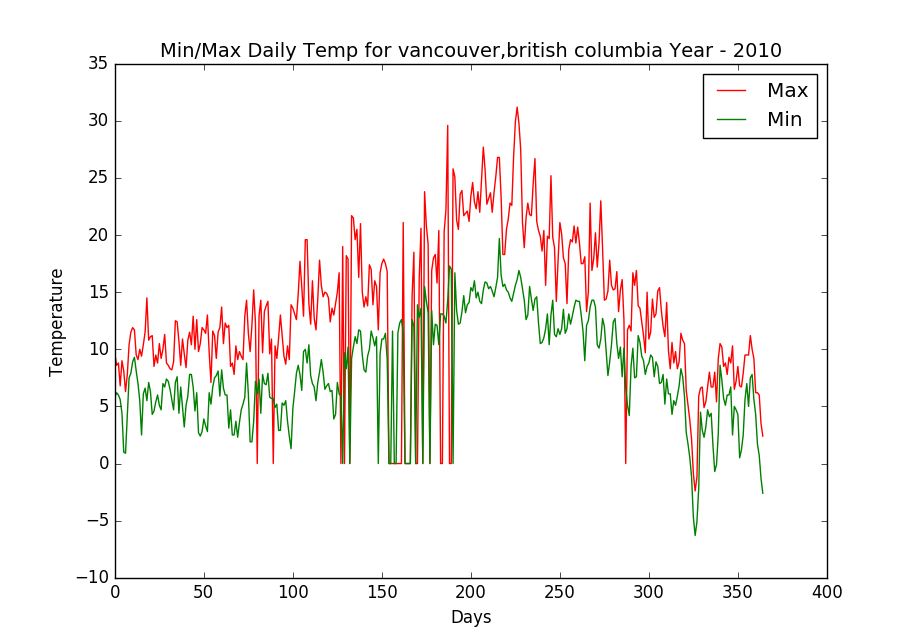
\includegraphics{Plot01.png}
%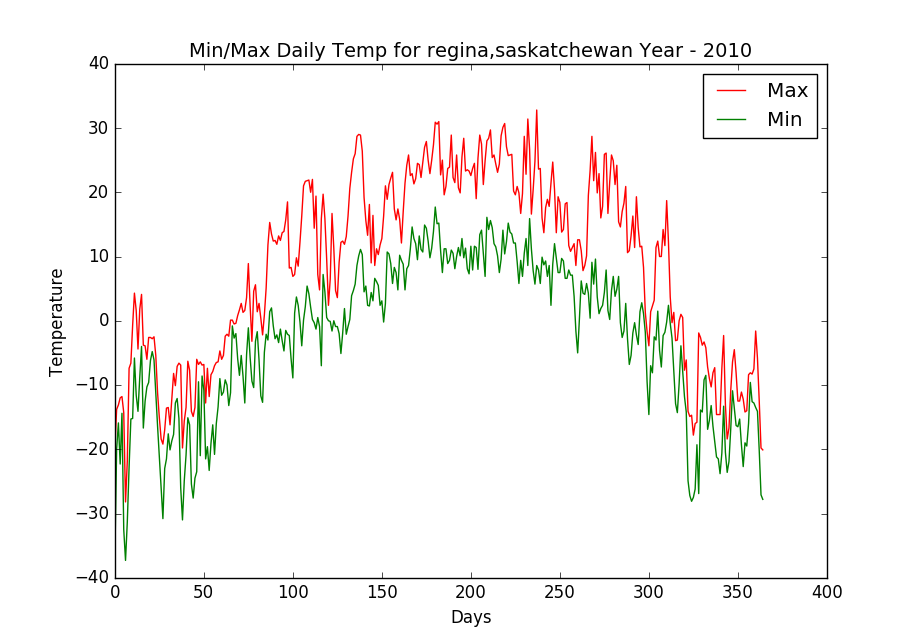
\includegraphics{Plot02.png}
%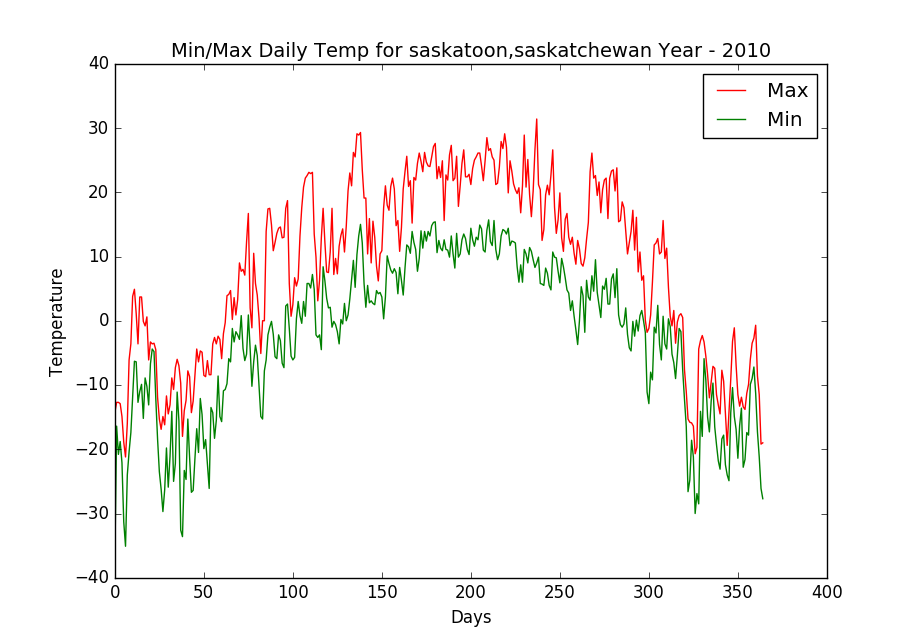
\includegraphics{Plot03.png}
%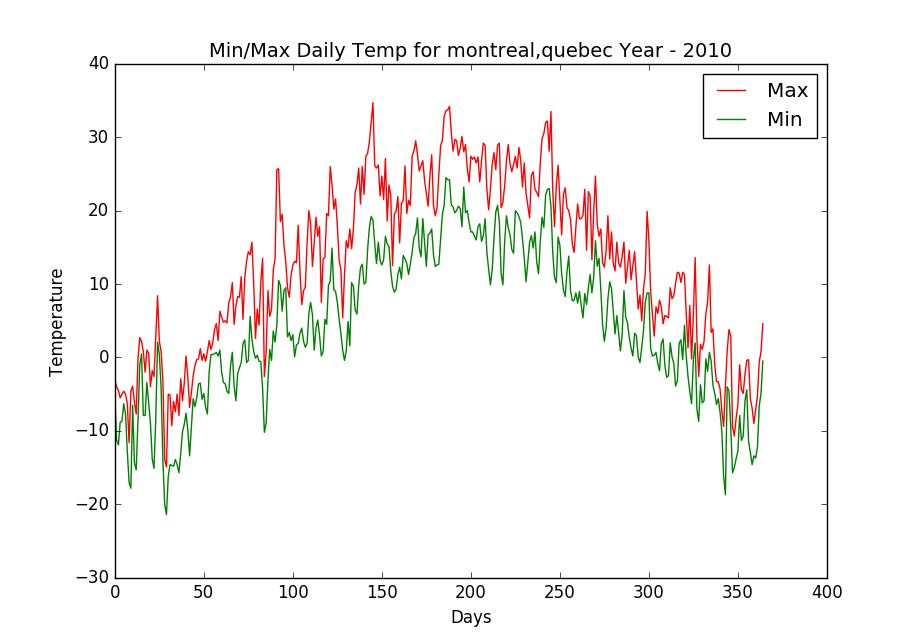
\includegraphics{Plot04.png}
%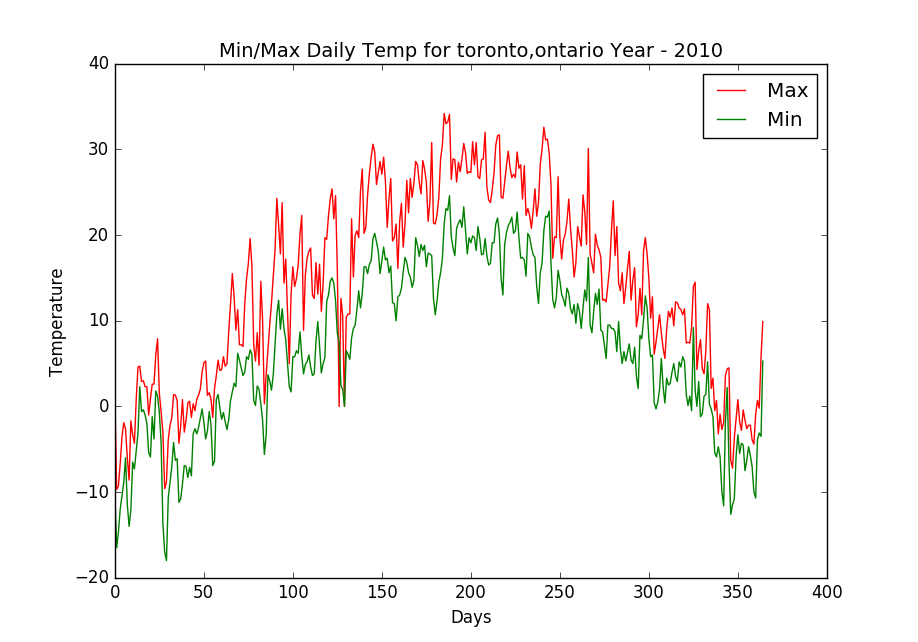
\includegraphics{Plot05.png}
\subsubsection{section}
\section{Experimental Results}
In our experiments, we used 
\subsection{result}
Parameter settings listed in table 1 was used for exploring the performance of 
\section{Discussion}
\section{Conclusion}
In this work ...
\newpage
\end{document}
